\chapter{Lineárne výrazy, rovnice a nerovnice}

\begin{example}
	V sčítacej pyramíde sa súčet čisel v susedných poličkách rovná číslu v políčku nad nimi. Ktoré číslo patrí v nasledujúcej sčítacej pyramíde na miesto otáznika?
	\begin{center}
		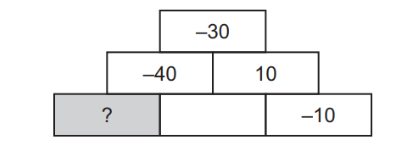
\includegraphics{assets/pyramida1.png}
	\end{center}
\end{example}

\begin{example}
	Pani Klára má v banke povolené prečerpanie účtu. Aktuálne je na jej účte mínusový zostatok -125,80 €. Po pripísaní výplaty sa suma na jej účte zmenila 721,50 €. Vypočítaj výšku výplaty pani Kláry v eurách.  
\end{example}

\begin{example}
	Jolana číta detektívku. Prečítala už 270 strán. Koľkostrán ma celá detektívka, ak Jolane zostáva prečítať $\frac{2}{5}$ detektívky.
\end{example}

\begin{example}
	Štyria súrodenci si sporia na spoločnú kolobežku. Tomáš nasporil o 30 € viac ako Eva, Roman dvakrát viac ako Eva a Soňa o 20\% viac ako Eva. Spolu už nasporili 290 €. Ktoré z nasledujúcich tvrdení je nesprávne?
	
	\begin{enumerate}
		\item Sestry nasporili menej ako ich bratia.
		\item Bratia nasporili 3-krát viac ako Soňa.
		\item Tomáš nasporil o 20 € viac ako Roman.
		\item Eva nasporila o 10 € ako Soňa.
	\end{enumerate}
\end{example}

\begin{example}
	Nájdi riešenie rovnice $6x - (2 - 2x) = 3(x-4)$.
\end{example}

\begin{example}
	Ktoré číslo nie je riešením nasledovnej nerovnice: $3 < 2(3x-9)$?
	
	\begin{enumerate}
		\item 6
		\item 5
		\item 4
		\item 3
	\end{enumerate}
\end{example}

\begin{example}
	Rieš nerovnicu $2x - 77 > 93$ a urči, koľko dvojciferných čísel je riešením tejto nerovnice.
\end{example}

\begin{example}
	Súrodenci Novákovci potrebovali odvážiť psov Birna a Astu. Psy odmietali pokojne sedieť na váhe, preto sa odbážili spolu s nimi tak, ako je znázornené na obrázkoch. Koľko kilogramov vážila Asta?
	
	\begin{center}
		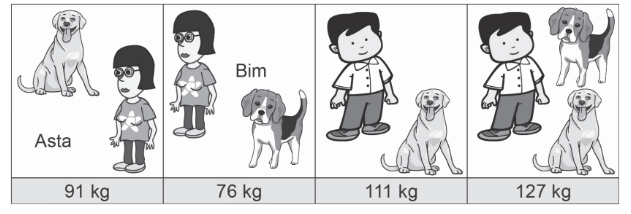
\includegraphics{assets/novakovci.png}
	\end{center}
\end{example}

\begin{example}
	Vypočítaj hodnotu výrazu $2x + 3(2 - y)$ pre $x = 3$ a $y = -1$.
\end{example}

\begin{example}
	Na ľavej strane rovnice je výraz $x - 2,4$. Zisti, ktorý z výrazov patrí na pravú stranu rovnice, aby rovnica mala koreň 2,8.
	
	\begin{enumerate}
		\item $3(x - 1,1)$
		\item $2(3 - x)$
		\item $3(x + 1,1)$
		\item $2(3 + x)$
	\end{enumerate}
\end{example}

\begin{example}
	Vyrieš rovnicu a výsledok uveď s presnosťou na stotiny: $11(x-1) = 11 - (1 + x)$.
\end{example}

\begin{example}
	Na školskom výlete x chlapcov. Dievčat bolo o 6 menej ako chlapcov. Dvojsedačkovou lanovkou sa všetci vyviezli z dolnej na hornú stanicu. Rozhodni, ktorý výraz vyjadruje počet sedačiek obsadených žiakmi, ak každá bola obsadené dvomi žiakmi.
	
	\begin{enumerate}
		\item $(x - 6) \div 2$
		\item  $(x - 6 + x - 6) \div 2$
		\item $(x + x) \div 2 - 6$
		\item $(x + x - 6) \div 2$
	\end{enumerate} 
\end{example}

\begin{example}
	Súčin troch čísel je 224. Prvé z nich je 10, druhé je 50-krát menšie ako prvé. Vypočítaj tretie číslo. 
\end{example}

\begin{example}
	Ktoré číslo treba doplniť na miesto otáznika tak, aby mala rovnica koreň 3? $2x - -3(5-x) - 1 = x - $ ?
\end{example}

\begin{example}
	Ktoré číslo má tú vlastnosť, že ak ho zväčšíme o 7, dostaneme číslo, ktoré má rovnakú absolútnu hodnotu ako toto číslo?
\end{example}

\begin{example}
	Nad každou dvojicou vedľa seba zobrazených výrazov na obrázku je ich súčet. Zistite, ktorý výraz bude na najvyššom mieste na obrázku.
	
	\begin{center}
		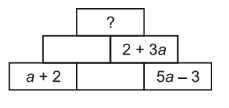
\includegraphics{assets/pyramida2.png}
	\end{center}
\end{example}

\begin{example}
	Urči číslo, ktoré je riešením rovnice $333 - 33x = 3$.
\end{example}

\begin{example}
	Tretina neznámeho čísla je rovnako veľká ako päťnásobok tohoto rozdielu tohoto neznámeho čísla a čísla 28. Urči toto neznáme číslo.
\end{example}

\begin{example}
	Môj pes je o 4,4 kg ťažší ako moja mačka. Spolu vážia 15 kg. Koľko váži môj pes?
\end{example}

\begin{example}
	Ktorý z výrazov má pre hodnotu $x = -3$ hodnotu 10?
	
	\begin{enumerate}
		\item $7 - x$
		\item $13 - x$
		\item $x - 13$
		\item $x - 7$
		
	\end{enumerate}
\end{example}

\begin{example}
	Ktoré najmenšie celé číslo je riešením nerovnice $0.5x - 7 < 2x - 50$?
\end{example}

\begin{example}
	Eugen má o 27 kníh viac ako Daniela, ale 3-krát menej ako Tomáš. Tomáš má 132 kníh. Koľko kníh má Daniela?
\end{example}

\begin{example}
	Pán Martin má v knižnici 150 kníh. Rozdelil ich do piatich kategórií. Románov je 75, encyklopédií je 5-krát menej ako románov. Detských kníh má o 4 viac ako cestopisov. V kategórii hobby si nechal 20 kníh. Koľko cestopisov má Martin vo svojej knižnici.
\end{example}

\begin{example}
	Vypočítaj hodnotu výrazu y pre = = -2 podľa nasledovnej schémy.
	
	\begin{center}
		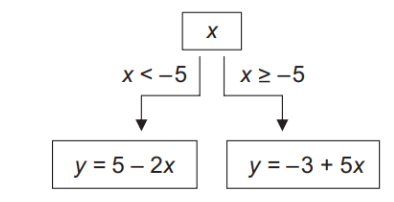
\includegraphics{assets/schema.png}
	\end{center}
\end{example}

\begin{example}
	V nasledujúcej tabuľke uvedený cenník listov kúpaliska.
	
	\begin{center}
		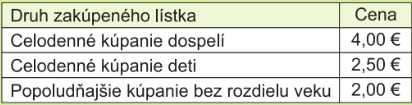
\includegraphics{assets/tab3.png}
	\end{center}
	
	Počas dňa si na kúpalisko kúpilo lístok $x$ dospelých a $y$ detí. Na popoludňajšie kúpanie sa predalo 17 lístkov. Ktorý výraz vyjadruje tržbu kúpaliska počas celého dňa?
	
	\begin{enumerate}
		\item $6,5xy + 17$
		\item $4x + 2,5y + 17$
		\item $4x + 2,5y + 34$
		\item $6,5xy + 34$
	\end{enumerate}
\end{example}